\documentclass[]{scrartcl}
\usepackage{listings}
\usepackage{graphicx}

%opening
\title{Exercise Sheet 4: Intel Cilk and OpenCL}
\author{Gaurav Kukreja, Evangelos Drossos}

\begin{document}
\lstset{language=C}

\maketitle

\begin{abstract}

\end{abstract}

\section{Exercise 11: Cilk and OpenCL}

\subsection{Advantages of Cilk and keywords needed}
Cilk is designed keeping in mind, that the developers and software producers
are not interested in rewriting the code, to exploit the benefits of parallelism.
Therefore it is designed in a way such that developers can exploit parallelism, by 
making small modifications to existing code. The resulting code continues to
perform on older machines with single processors, and makes us of parallel hardware
whenever possible.

Using Cilk is easier compared to other parallel programming constructs and frameworks.
It supports 3 keywords \textit{\_cilk\_spawn}, \textit{\_cilk\_sync} and \textit{\_cilk\_for}.

\subsubsection{cilk\_spawn}
This keywords modifies a function call statement to tell the runtime system that
the function may(but is not required to) run in parallel with the caller. This keyword
may be used as follows

\begin{lstlisting}
type var = cilk_spawn (func args) ; // func () returns a value
var = cilk_spawn func(args) ; // func () returns a value
cilk_spawn func(args) ; // func() may return void
\end{lstlisting}

\subsubsection{cilk\_sync}
The cilk\_sync statement indicates that the current function cannot continue in parallel with its
spawned children. After the children all complete, the current function can continue.

\begin{lstlisting}
cilk_sync;
\end{lstlisting}

This statement only syncs with children spawned by this function. Children of other functions are not affected.

\subsubsection{cilk\_for}
A cilk\_for loop is a replacement for the normal C/C++ for loop that permits loop iterations 
to run in parallel. The syntax is as follows

\begin{lstlisting}
cilk_for(declaration; 
		conditional expression; 
		increment expression)
body
\end{lstlisting}

There are some restrictions to use of cilk\_for. The loop must be simple, with uniform
stride length. The control variable, or iteration counter must not be changed inside the 
loop, other than in the increment expression of the cilk\_for statement. The termination
condition should be simple, and should not change between iterations.

\pagebreak
\subsection{Array Expressions with Intel C language extensions}
C/C++ language extensions for array notations is an Intel-specific language extension 
that is part of Intel Cilk Plus feature supported by Intel Compiler. The extension provides
following major benefits:

\begin{enumerate}
	\item Allows use of array notations to program parallel operations
	\item Achieves predictable performance based on mapping parallel constructs to the underlying multi-threaded and SIMD hardware.
	\item Enables compiler parallelization and vectorization with less reliance on alias and dependence analysis.
\end{enumerate}

\subsubsection{Array Section Notation}
A new section operator is introduced. 

\begin{lstlisting}
section_operator ::= [<lower_bound> : <length> : <stride>]
\end{lstlisting}

Here, \textit{lower\_bound}, \textit{length} and \textit{stride} are integers. The statement
represents a set of integer values as follows

\begin{verbatim}
<lower_bound>, <lower_bound + stride>, <lower_bound + 2*stride>,
 ... , <lower_bound + (length-1)*stride>
\end{verbatim}

A section operator can occur in place of a subscript operator. That is, elements of an array
a[lb], a[lb+str], a[lb+2*str], ..., a[lb + (len-1)*str] can be represented as a[lb:len:str].
Further usage of the section operator is illustrated as follows:

\begin{lstlisting}
a[0:3][0:4]	// refers to 12 elements in the 2-dimensional
		array starting at row 0, column 0, and ending
		at row 2,column 3
b[0:2:3] 	// refers to elements 0 and 3 of 1 dimensional
		array b
b[:] 		// refers to the entire array b
\end{lstlisting}

\subsubsection{Types of expressions}

\begin{itemize}

\item \textbf{Operators} \\
	Most C/C++ operators are available for array sections. Following expressions can be used.
	
	\begin{lstlisting}
a[:] * b[:]	//element-wise multiplication
a[0:3][0:3] + b[1:4][1:4] // matrix addition
a[0:3][0:3] + b[0][1] // allowed. adds scalar b[0][1] to an
	array section.
	\end{lstlisting}

	Operations between sections of different size will fail.

\item \textbf{Assignment} \\
	Assignment operator applies in parallel to every element of the array section.
	
	\begin{lstlisting}
a[0:3] = b[0:3] + c;
a[:][:] = d[:]; // error, different rank
	\end{lstlisting}

\item \textbf{Gather and Scatter} \\
	When an array section occurs directly under a subscript expression, it designates a set of elements indexed by the values of the array section.
	
	\begin{lstlisting}
unsigned index[10] = {0,1,2,3,4,5,6,7,8,9};
float out[10], in[10] = {9,8,7,6,5,4,3,2,1,0};
out[0:5] = in[index[0:5]]; // gather
out[index[5:5]] = in[0:5]; //scatter
for(int i = 0; i < 5; i++){
	cerr << "out[" << i << "]" << out[i] << endl;
}
	\end{lstlisting}

	\item \textbf{Reduction Operations} \\
	There are some built in Reduction functions which use the section operator e.g. 
	\textit{\_\_sec\_reduce\_add (a[:])}, which adds the values passed as arrays, and
	returns result. Similarly, following reduction functions are built-in.
	\begin{itemize}
		\item \texttt{\_\_sec\_reduce\_mul (a[:]) // multiplies all values in array}
		\item \texttt{\_\_sec\_reduce\_all\_zero (a[:]) // checks if all values are 0}
		\item \texttt{\_\_sec\_reduce\_all\_nonzero (a[:]) // checks if all values are not 0}
		\item \texttt{\_\_sec\_reduce\_any\_nonzero (a[:]) // tests for a value that is not 0}
		\item \texttt{\_\_sec\_reduce\_min (a[:] // returns minimum value}
		\item \texttt{\_\_sec\_reduce\_max (a[:])// returns maximum value}
		\item \texttt{\_\_sec\_reduce\_min\_ind (a[:]) // returns index of min value}
		\item \texttt{\_\_sec\_reduce\_max\_ind (a[:]) // returns index of max value}		
	\end{itemize}
	
	\item \textbf{Shift Operations}
	Intel Cilk PLus supports shift and rotate operations on array sections. The function
	prototypes are as follows
	
	\begin{lstlisting}
b[:] = __sec_shift(a[:], signed shift_val, fill_val) // Generic Shift Function
b[:] = __sec_rotate(a[:], signed shift_val) // Generic Rotate Function
	\end{lstlisting}
	
	\item Function Maps
	Maps are implicitly defined on scalar functions. They take array sections, and run on
	each element in parallel, with no specific ordering. For example,
	
	\begin{lstlisting}
a[:] = sin(b[:]);
a[:] = pow(b[:], c);
a[:] = pow(c, b[:]);
	\end{lstlisting}
\end{itemize}
	
\pagebreak
\subsection{Memory Structure in OpenCL}
OpenCL is a framework for exploiting parallel hardware found in CPUs, GPGPUs and
other special hardware. Unlike CUDA, OpenCL is designed to be compatible with a vast
variety of hardware. Therefore, OpenCL assumes a uniform hardware architecture for
the sake of its execution and memory model. The appropriate features provided by the
hardware are mapped to this architecture by the run-time system.

The following figure shows the hardware architecture assumed by OpenCL.

\begin{figure}[hb]
	\centering
	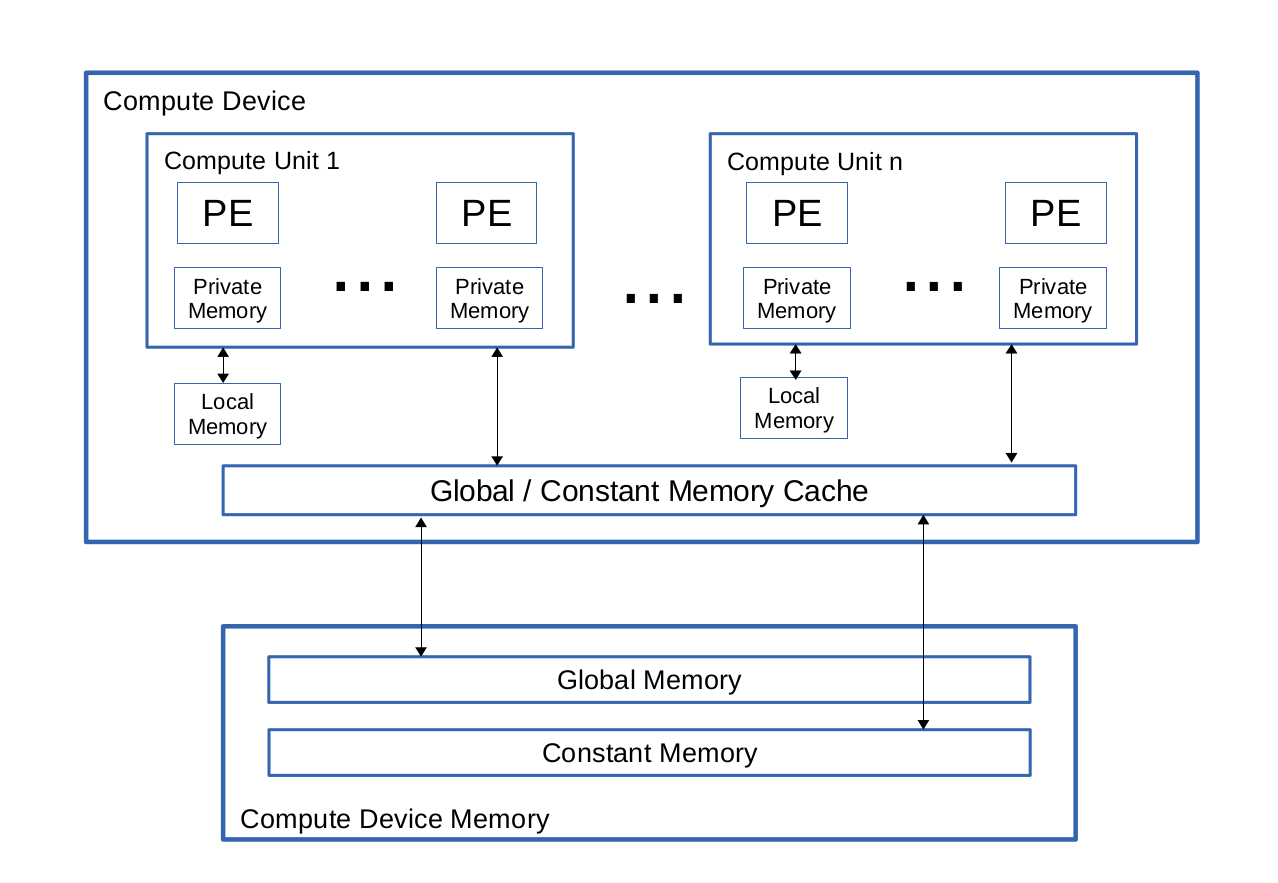
\includegraphics[width=0.8\textwidth]{opencl_memory}
	\caption{Memory and Hardware Structure in OpenCL}
\end{figure}

Let's consider GPGPUs for our reference Compute Device. The Compute Device consists of
several Compute Units (Arithmetic Logical Units that execute code). The Compute Device has
Global Memory, which can be accessed by all the compute units in the device. This is a high
latency memory. This memory can also be accessed by the Host Device (CPU). The host device
communicates with the Compute Device using this memory.

The Device also has a low latency Constant Memory. Like Global Memory, this memory can also
be accessed by all Compute Units, but none of the Compute Units can write to this memory. 
Only the Host (CPU) will write to this memory. This memory can be used to provide input data
which does not need to be modified during the execution of code. The actual hardware may not
have the Constant Memory, in which case the run-time system will simply use the Global Memory.

The device has a Global/Constant Memory Cache. The content of this memory cannot be directly
controlled by the Compute Units. This is low latency cache memory which is maintained by the
run-time system.

Local Memory is a low latency memory, which is private to each Compute Unit. One Compute Unit
may not access contents in another Units Local Memory. OpenCL provides programmers with the
facility to designate data that needs to be held in Local Memory. The actual hardware may not
have Local Memory, or may have only a small amount of Local Memory. In this case, the data will
be stored in Global Memory. 

For best results, the user must customize the code such that optimal use of the hardware
resources can be achieved.

\pagebreak
\subsection{OpenCL Execution Model and Compilation of OpenCL Application}
An OpenCL application consists of 2 parts
\begin{itemize}
	\item Device Code
	\item Host Code
\end{itemize}
Host code runs on the Host Device eg. CPU. The host code is compiled by a standard C
compiler like GCC. The host code contains boiler plate code, which is used to detect the
hardware available on the system, and check the features. The host code initializes the
hardware to be used. It then creates the executable device code. As per the application
demands, the kernel along with input data is transferred to the Compute Device and execution
is started. The Host then reads the result from the Compute Device.

The Device Code is written in a language very similar to C, but with some extra features
and some restrictions. Special hardware specific compilers are used to compile the Device Code.
The compiled Device code is called the kernel. The host code detects hardware(GPGPUs) on the 
system and selects an appropriate hardware. It then tries to find the corresponding compiler,
and compiles the Device Code to create the kernel.

\pagebreak
\section{Exercise 12: Quicksort with Intel Cilk}

\subsection{Code Overview}
For this exercise, we implemented the quicksort algorithm using Intel Cilk Plus. 
Since quicksort works in a recursive manner, we used the \textit{\_cilk\_spawn} keyword to spawn 
new threads and parallelize the computation for the left and right subarrays. 
The \textit{\_cilk\_sync} keyword helped us synchronize the children of the function at a given level 
of recursion. 
Following code fragment shows how our implementation works:
	\begin{lstlisting}
/* recursion */
cilk_spawn quicksort(data, right);
quicksort(&(data[left]), length - left);
cilk_sync;
	 \end{lstlisting}

\subsection{Results and Analysis}
We designed a number of tests to measure the performance of our implementation. We performed both weak and strong scaling for different problem sizes. Furthermore, we compared the performance of the Intel Cilk Plus Implementation with our OpenMP implementation from the second assignment.

Following figure shows the speedup achieved for different numbers of threads for the Intel Cilk implementation. Results are shown for three problem sizes: an array length of 4, 8 and 16 million elements. 

\begin{figure}[hb]
	\centering
	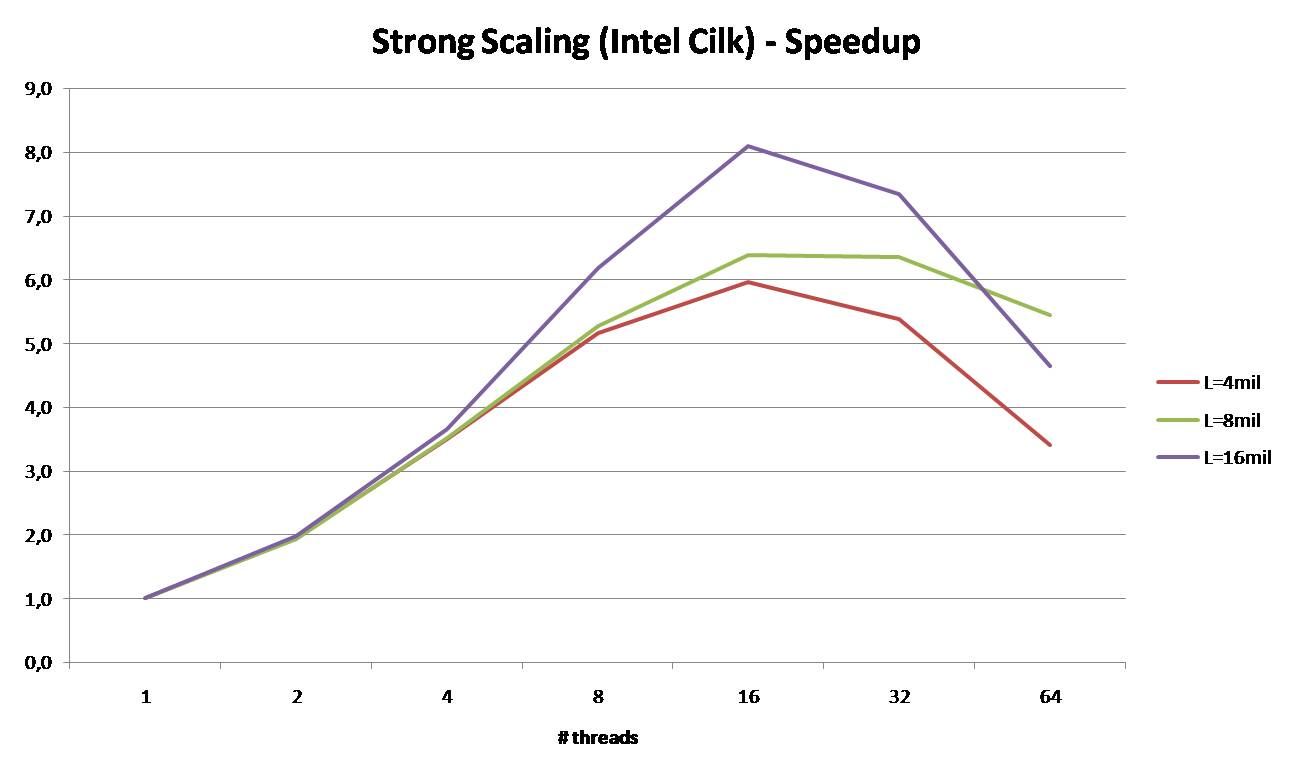
\includegraphics[width=0.8\textwidth]{Cilk_speedup}
	\caption{Speedup of Intel Cilk Plus implementation for three different problem sizes}
\end{figure}

As can be seen in figure 2, the highest speedup is achieved for 16 threads. After this point, performance levels off and a steep decline is visible for 64 threads. This is due to the additional overhead, since the maximum number of threads for this partition has been exceeded. 
Speedup seems to be slightly better for larger problem sizes. It should also be noted that doubling the number of threads leads to less than twice as good performance, but performance improvements are still large.

The next figure compares the Intel Cilk variant of quicksort to the OpenMP implementation of the algorithm. It is immediately clear that both implementations achieve almost the same performance. The highest performance gain is achieved for 16 threads.

\begin{figure}[hb]
	\centering
	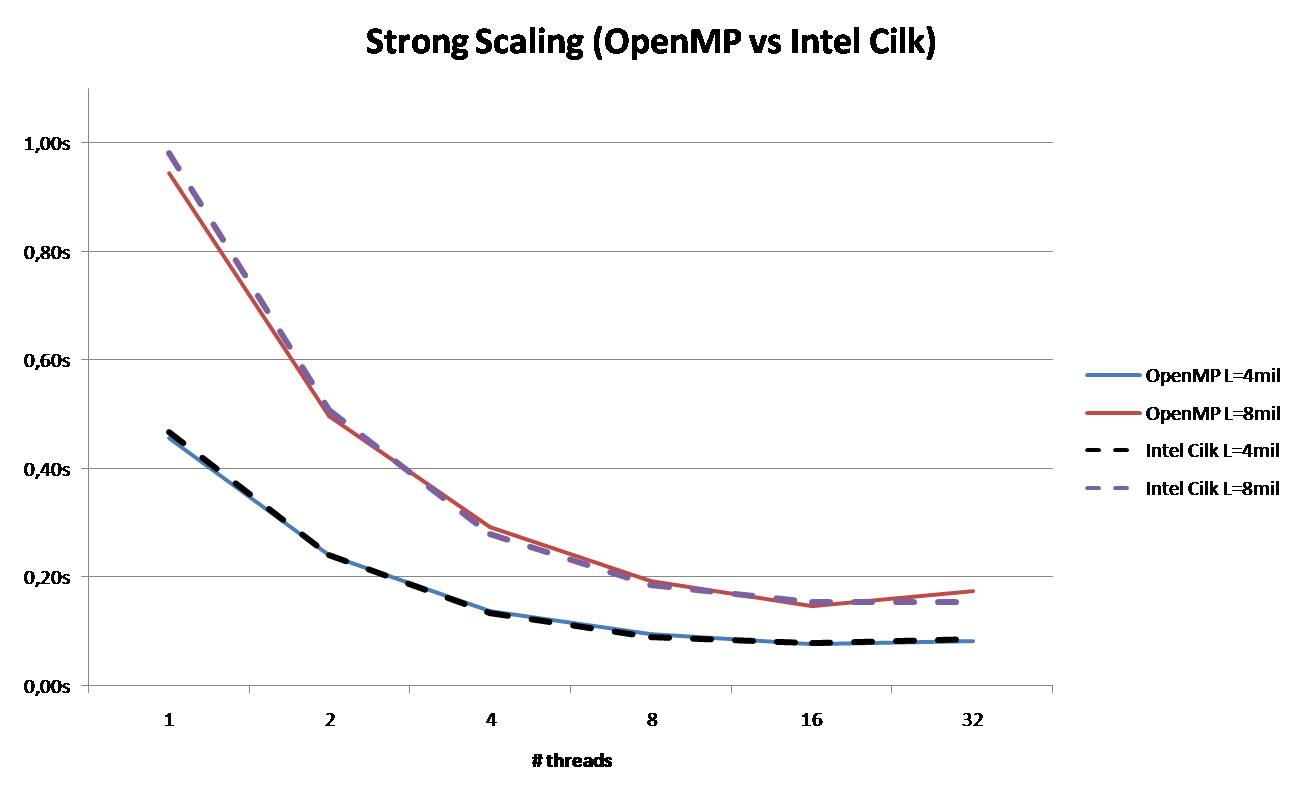
\includegraphics[width=0.8\textwidth]{quick_strong_scaling2}
	\caption{Strong scaling comparison for Intel Cilk and OpenMP implementations of quicksort. The vertical axis shows time elapsed in seconds and the horizontal axis the number of threads used}
\end{figure}


Lastly, we also attempted a number of weak scaling tests to compare both implementations. We started with a problem size of 1 million elements and 1 thread and iteratively doubled both problem size and the number of threads up to a cumulative factor of 32.

\begin{figure}[h!]
	\centering
	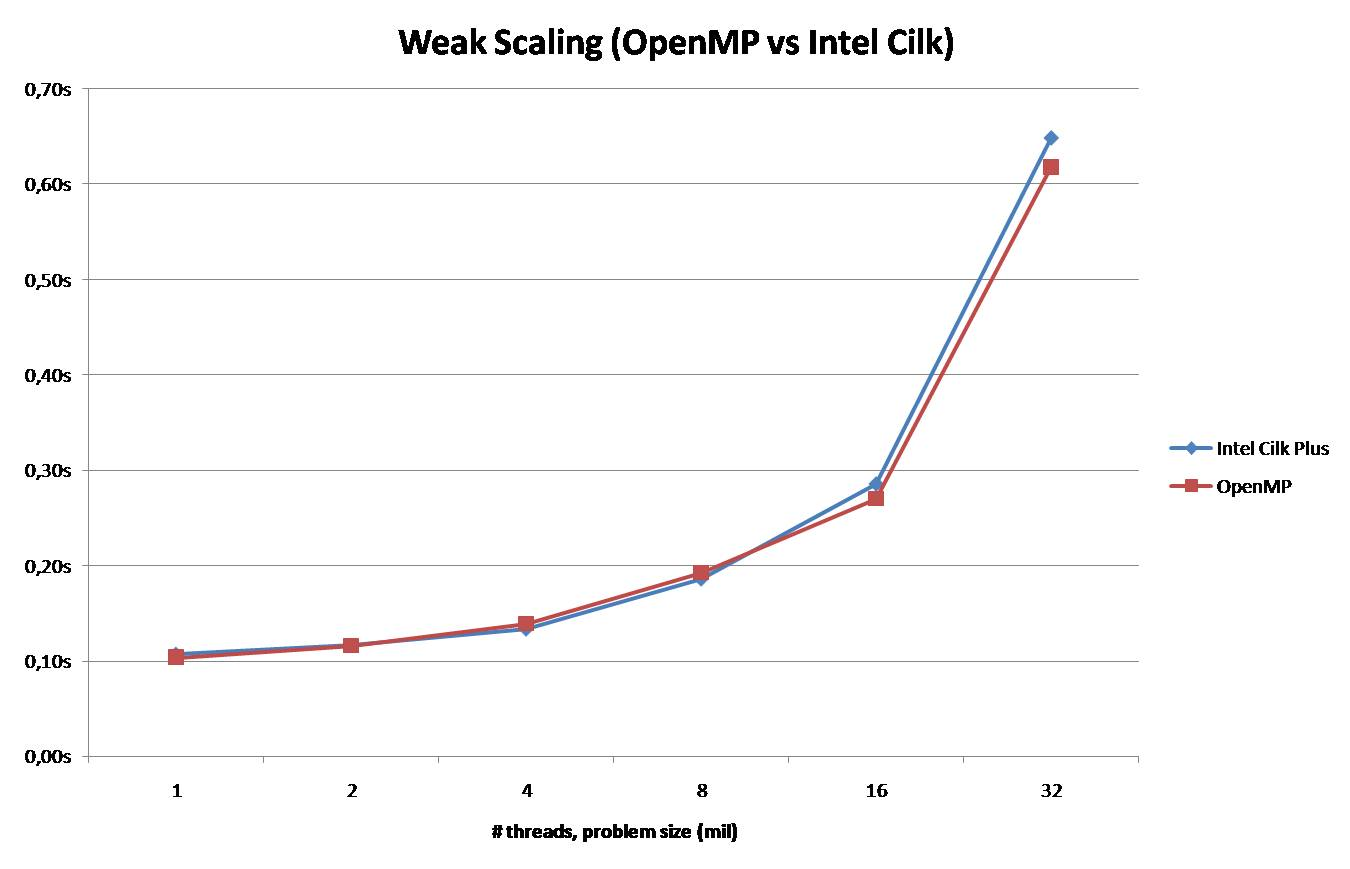
\includegraphics[width=0.8\textwidth]{quick_weak_scaling}
	\caption{Weak scaling comparison for Intel Cilk and OpenMP implementations of quicksort. The vertical axis shows time elapsed in seconds and the horizontal axis the number of threads spawned as well as the array length in million elements}
\end{figure}

As demonstrated by figure 4, performance is almost identical. At first, elapsed time does not change much at each step. However, at 16 threads the needed time is already almost 3 times the time needed for initial problem of 1 million elements running on one thread. From that point onwards the problem does not scale very well.

\pagebreak
\section{Exercise 13: Laplace Equation with Intel Array Extensions}

\subsection{Code Overview}
For the Laplace Equation Solver we implemented two versions using the Intel Array Extensions (IAE) and another one using pragma notation for the stencil operation and IAE in all other routines.
Our first implementation using IAE utilizes one dimensional arrays to annotate two dimensional matrices. In the original (serial) implementation of the algorithm nested for loops were used to access a section of a matrix row. We treated those parts of the code in a similar way, by replacing only the inner loop through the array notation extensions and keeping the outer loop in place.
This approach can be demonstrated in following example showing the \textit{g\_scale} function:

\begin{lstlisting}
void g_scale(double* grid, double scalar)
{
	
	int start;
		
	for (int i = 1; i < grid_points_1d-1; i++)
	{
		start = ((i*grid_points_1d) + 1);
		grid[start:(grid_points_1d-2)] = grid[start:(grid_points_1d-2)] * scalar;
	}
	
}
\end{lstlisting}

We followed a rather different approach in the \textit{iae2\_poisson.cpp} version of the algorithm. In this case we trasnformed one-dimensional arrays to two dimensional ones (wherever applicable) and used intel array extensions to replace inner and outer loops.

Finally, as already mentioned, we implemented a third version of this algorithm where we denoted the stencil operation using the simd vectorization pragma.  

\subsection{Results and Analysis}
We performed a number of tests to determine the performance of the respective algorithms for different problem sizes. As one can see in the following figure, the best performing implementation is by far the one using Intel Array Extensions on two-dimensional arrays. This was to be expected, since the transformation of 1d into 2d arrays allowed the compiler to fully exploit vectorization options. The pragma simd and the one-dimensional array IAE implementanion show similarly weak performance, especially for larger problem sizes.

\begin{figure}[hb]
	\centering
	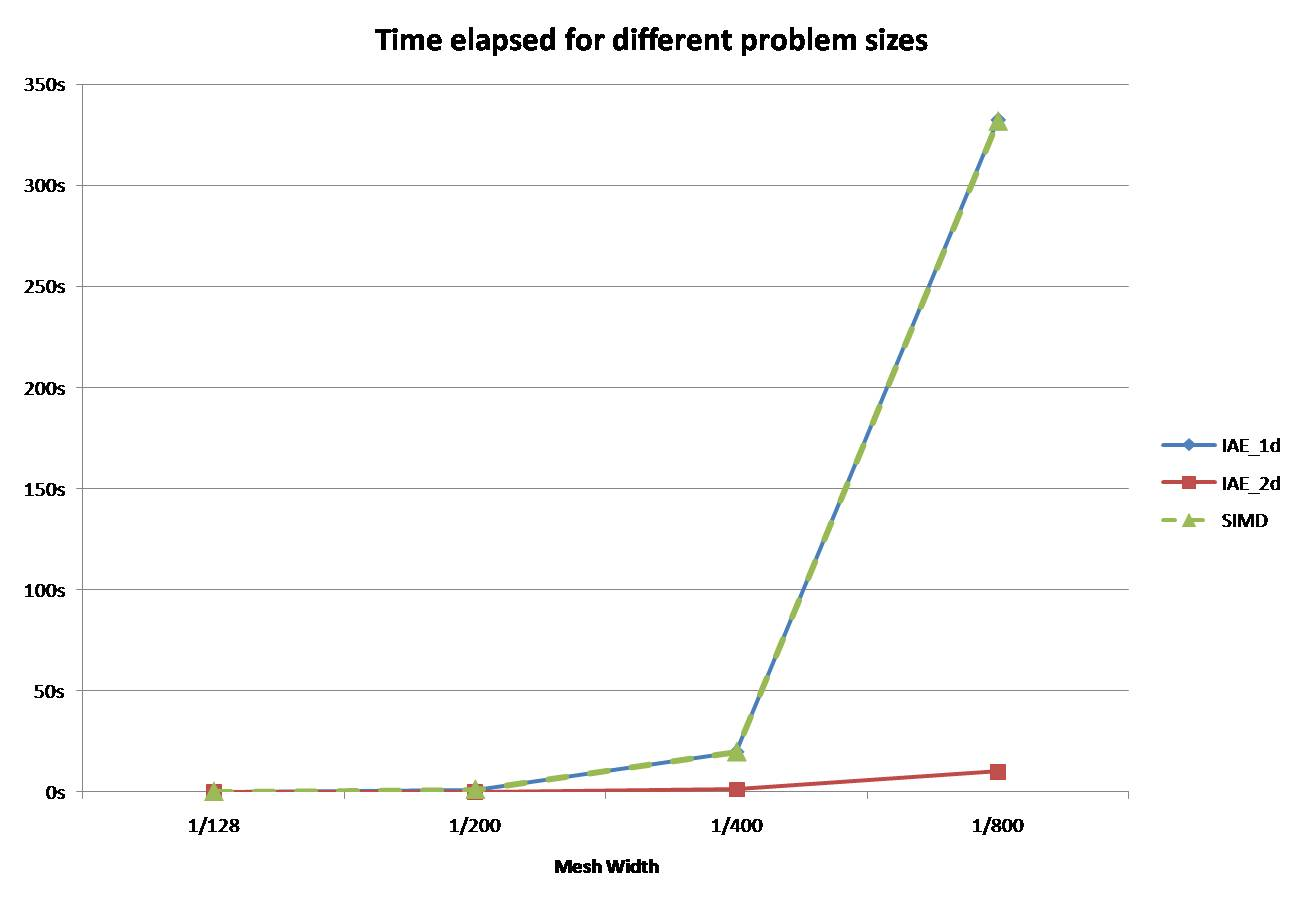
\includegraphics[width=0.8\textwidth]{poissonIAE_time}
	\caption{Performance comparison of the three laplace solver implemenations. Time elapsed is given in seconds and the x-axis denotes mesh width. The maximum number of iterations was set high enough so that it would not be reached during runtime and the accuracy was set in all cases to 0.0001}
\end{figure}


\pagebreak
\section{Exercise 14: Matrix Multiplication with OpenCL}

\subsection{Overview}
We were able to achieve Matrix Multiplication using OpenCL with Local Memory Blocking Optimization.
Further details of our implementation are discussed below.

The project consists of 2 files.
\begin{itemize}
	\item \textbf{main\_benchmark.c} - Host Code
	\item \textbf{matrix\_mul\_kernel.c} - Device Code
\end{itemize}

\subsection{Algorithm}
A simple implementation of Matrix Multiplication creates a 2 dimensional array of threads, one for
each element of the product matrix. Each thread calculates the value of the element that it corresponds to. The threads are divided into Work Groups which run in parallel on the Compute Units
in the device. Each Compute Unit has a number of Processing Elements, which process the Work Items
(threads) in parallel. Each thread can be uniquely identified with combination of \textit{global} and \textit{local} ids in each dimension, which can be used to identify which element of the product
matrix the thread must evaluate.

As can be easily seen, the simple approach is suboptimal. The Computational Intensity of this approach is very low. For a matrix of width 1024, each thread performs 2048 Reads, 1024 Floating Point Multiplications, 1024 Floating Point Additions and 1 Write operation. If we are able to reduce the number of read operations from global memory, by making use of the Local Memory, we can optimize the performance. 

The Local Memory on the GPUs connected to Linux Cluster is 32 KB. We can store 3 matrices of width 32 in this memory, while still keeping space for temporary variables. In our approach, we divide
matrices into square blocks of width 32. Each work group correspondingly is also a square matrix of width 32 i.e. it has 32x32 threads. 

Each thread in a Work Group reads one element from each input matrix from Global Memory
and stores it into Local Memory. Now we have the entire block of size 32x32 in low latency Local Memory. Each thread computes the partial result for its corresponding element in the product matrix
from these values. This way, each thread performs 2 Read operations, 32 Floating Point
Multiplications, 32 Floating Point Additions and 1 Write operation for calculating the partial result. The computational intensity of this approach is almost 32 times better than the simple approach.

\subsection{Results and Analysis}
When talking about performance results from OpenCL, care must be taken to understand that apart from the processing time,
a lot of overhead is spent in compiling the kernel sending the data to the Global Memory of the GPU, and reading the results
back from the GPU. 

Our results show a very  high performance if we consider only time spent to compile the kernel. This is expected, owing to high
parallelism of an application like Matrix Multiplication, and the large number of small cores on the GPU. Following image is the
graphic of the result considering only the time used to execute the kernel.

\begin{figure}[h!]
	\centering
	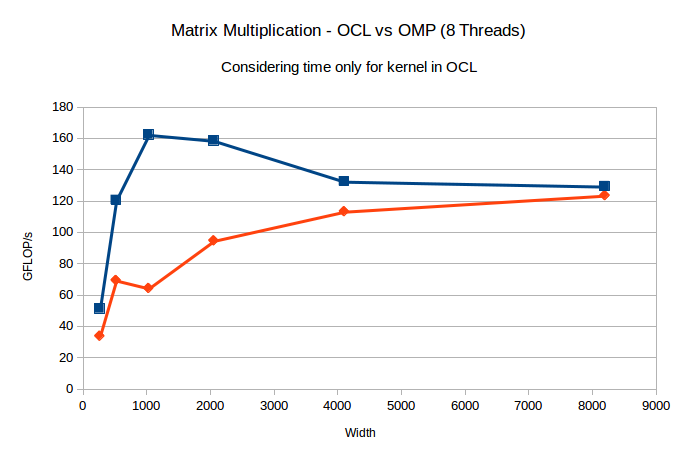
\includegraphics[width=0.8\textwidth]{mat_mul_ocl_vs_omp_kernel}
	\caption{\textbf{Comparison of GFLOP/s achieved for Matrix Multiplication.} Blue line depicts performance using OpenCL,
		and Orange line depicts performance with OpenMP. We consider only time spent in executing the kernels.}
\end{figure}

The performance steeply degrades when we consider the overhead spent in compiling the kernel, sending the input data to the GPU
and reading the output back from the GPU memory. Following image shows the result keeping this overhead in consideration.

\begin{figure}[h!]
	\centering
	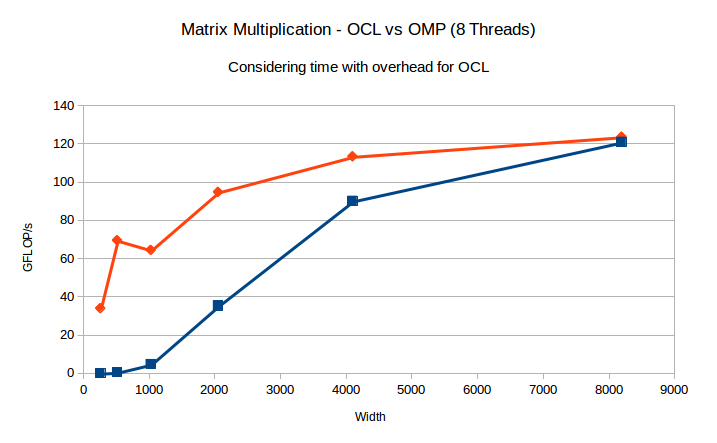
\includegraphics[width=0.8\textwidth]{mat_mul_ocl_vs_omp_overhead}
	\caption{\textbf{Comparison of GFLOP/s achieved for Matrix Multiplication with overhead.} Blue line depicts performance using
		OpenCL, and Orange line depicts performance with OpenMP. Here, we consider the total time spent in compiling kernels,
		transferring input matrices to GPU, execution of kernels and reading output matrix from GPU.}
\end{figure}

You can also observe that performance with OpenCL nearly matches performance with OpenMP at larger width. The impact of the overhead
is less when the problem size is large.

The OpenMP implementation used for this analysis, is running on 8 cores. It is optimized for Memory Blocking and uses Intel
Compiler Intrinsics features to facilitate vectorization.

\pagebreak
\section{Exercise 15: Laplace Equation with OpenCL}

\subsection{Code Overview}
The challenging aspect in trying to parallelize Laplace Equation Solver with OpenCL, is to efficiently parallelize the 
\textit{g\_product\_operator()} and \textit{g\_dot\_product()} functions.

We could correctly parallelize the \textit{g\_product\_operator()} function. We create one thread for calculating each element
of the result matrix. Further optimizations are possible, but unfortunately we could not invest enough time into it.

We tried to parallelize \textit{g\_dot\_product()} function, but failed. We created one thread for each row of the matrix. Each
thread calculates the scalar product of the row vectors of the matrix. Later, we try to reduce the value calculated by each
thread. We somehow could not fix some bug with reduce functionality. We could get the reduce functionality to work in a sample
application trial.cpp (included in source), but simillar code does not work for the real implementation. We will continue to give
more time to this.

\subsection{Results and Analysis}
We think that OpenCL is not an ideal choice for parallelizing this application. The kernels are small, and the overhead spent
in compiling kernels, and transferring data between GPUs is very expensive. This is also what is being reflected in the results we
have received. However, it must be noted that our results are with only \textit{g\_product\_operator()} function parallelized. 

Possibly, there are more avenues to exploit parallelism but we could not get time to check them.

The results with only \textit{g\_product\_operator()} function parallelized are as follows.
\begin{center}
	\begin{tabular}{|l | c | c|}
		\hline
		Problem Size & Serial (time) & OpenCL (time) \\ \hline
		512 & 0.26554 s  & 0.369021 s  \\ \hline
		1024 & 0.038892 s  & 0.351882 s  \\ \hline
		2048 & 0.390686 s  & 0.055191 s  \\
		\hline
	\end{tabular}
\end{center}

As can be seen from these results, we got a lot of random times. These times reported here are average times over a set
of runs. We could not clearly understand the reason for the trends.

\end{document}